\section{\toolname: Secure Messaging}
\label{sec:secureMessage}


\begin{figure*}[t]
 \centering
 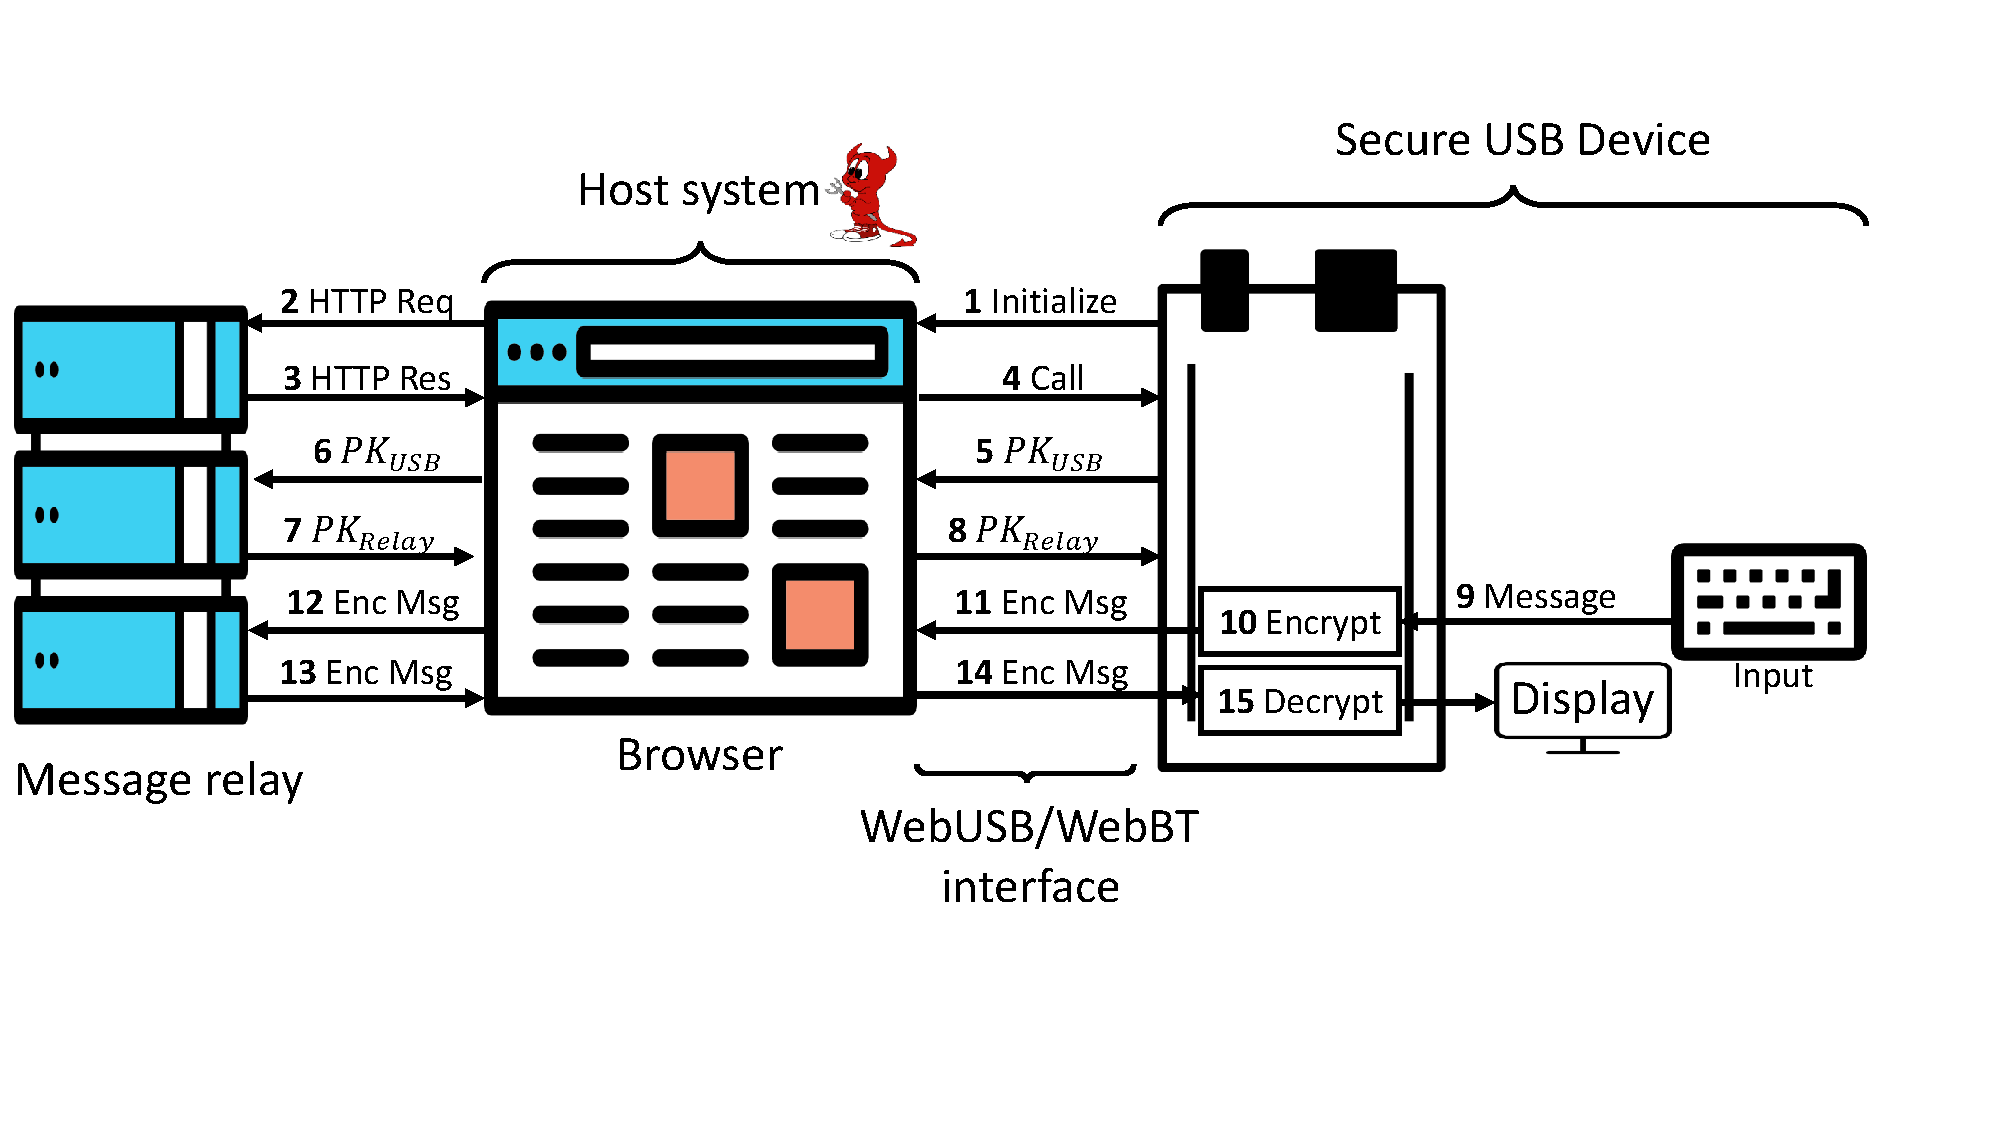
\includegraphics[trim={0 4cm 3cm 0},width=\linewidth]{SystemDesign_Dev2Dev.pdf}
 \caption{System design of the secure messaging using a semi trusted relay server. Steps $1-4$ denotes how the user loads a webpage from the relay server that serves \js snippet with \webusb/\webbt API. Steps $5-8$ shows establishment of the \ssl/\tls channel using the browser as an untrusted transport. $PK_{USB}$ and $PK_{Relay}$ are the public key corresponding to the secure \usb device and the message relay server respectively. Steps $9-12$ shows how the users type message on the input peripheral connected to the \usb device that transfer the message securely to the relay and receives encrypted message from the relay.}
 \label{fig:systemDesignDedicated}
\end{figure*}


The \webusb standard provides a way for the \js code served from a \https server to communicate with a \usb device. We leverage the secure channel established between the secure \usb device and the remote web server to establish an end-to-end encrypted messaging service. Such messaging service is aimed for the strongest attacker who can compromise the host systems, networks (ISP) and the in some cases the well known messaging service in terms of some dedicated back-door or flaw in the implementation (e.g. WhatsApp, Signal, Telegram etc.). We propose two different solutions for hardware backed messenger device based on the trusted \usb device which provides secure and authenticated input to the remote entity.

%Based on this we proposed a system where users can detect a phishing attack and securely provide credentials and sensitive inputs to the trusted remote web server even if the host is compromised by a global-network level attacker. 

\subsection{System model} 
\label{sec:secureMessage:systemModel}
Our system model primarily involves four parties. The \usb/\bluetooth enabled peripheral (keyboard, mice, bulk storage or any peripheral devices), a host which is a computer/smartphone which connects to the remote server, the aforementioned remote server (message relay) where the host is connected to and lastly a secure \usb/\bluetooth device that converts any generic \usb/\bluetooth peripherals to secure peripheral. The general settings assume that the peripherals are connected to the secure device devices which are connected to the host system. The connection could be wired or wireless depending on the case if the host system is a computer or a smartphone. Similarly, the communication between the secure device and the peripheral can be carried out by wired or wireless channel depending on the nature of the peripherals. The system model is independent of the physical connection between the host, secure device and the peripherals. 
%Our designed secure device is a small embedded device with very small TCB (few thousand lines of code) yet computationally powerful to carry out cryptographic operation efficiently.



The goals of our proposed system are the following:
\begin{enumerate}
  \item The secure USB/Bluetooth device has very small footprint i.e., extremely small trusted computing base (TCB). Also, the solution hardware should be very simple so it does not open additional attack vectors such as the vulnerability in complex operating system or browser program. This ensures minimal trust assumption.
  
  \item The solution should provide privacy against the strongest attacker model i.e., an attacker who is capable of compromising the entire network and the host system. The solution provides protection against local and remote phishing attacker, provides data (sensitive user input) confidentiality and authenticity.
 
  \item The secure device should be resilient against side-channel attacks such as power, timing analysis etc. 
  
%  \item All these functionalities are achieved with the addition of minimal delay.

\end{enumerate}



\begin{figure*}[!t]
 \centering
 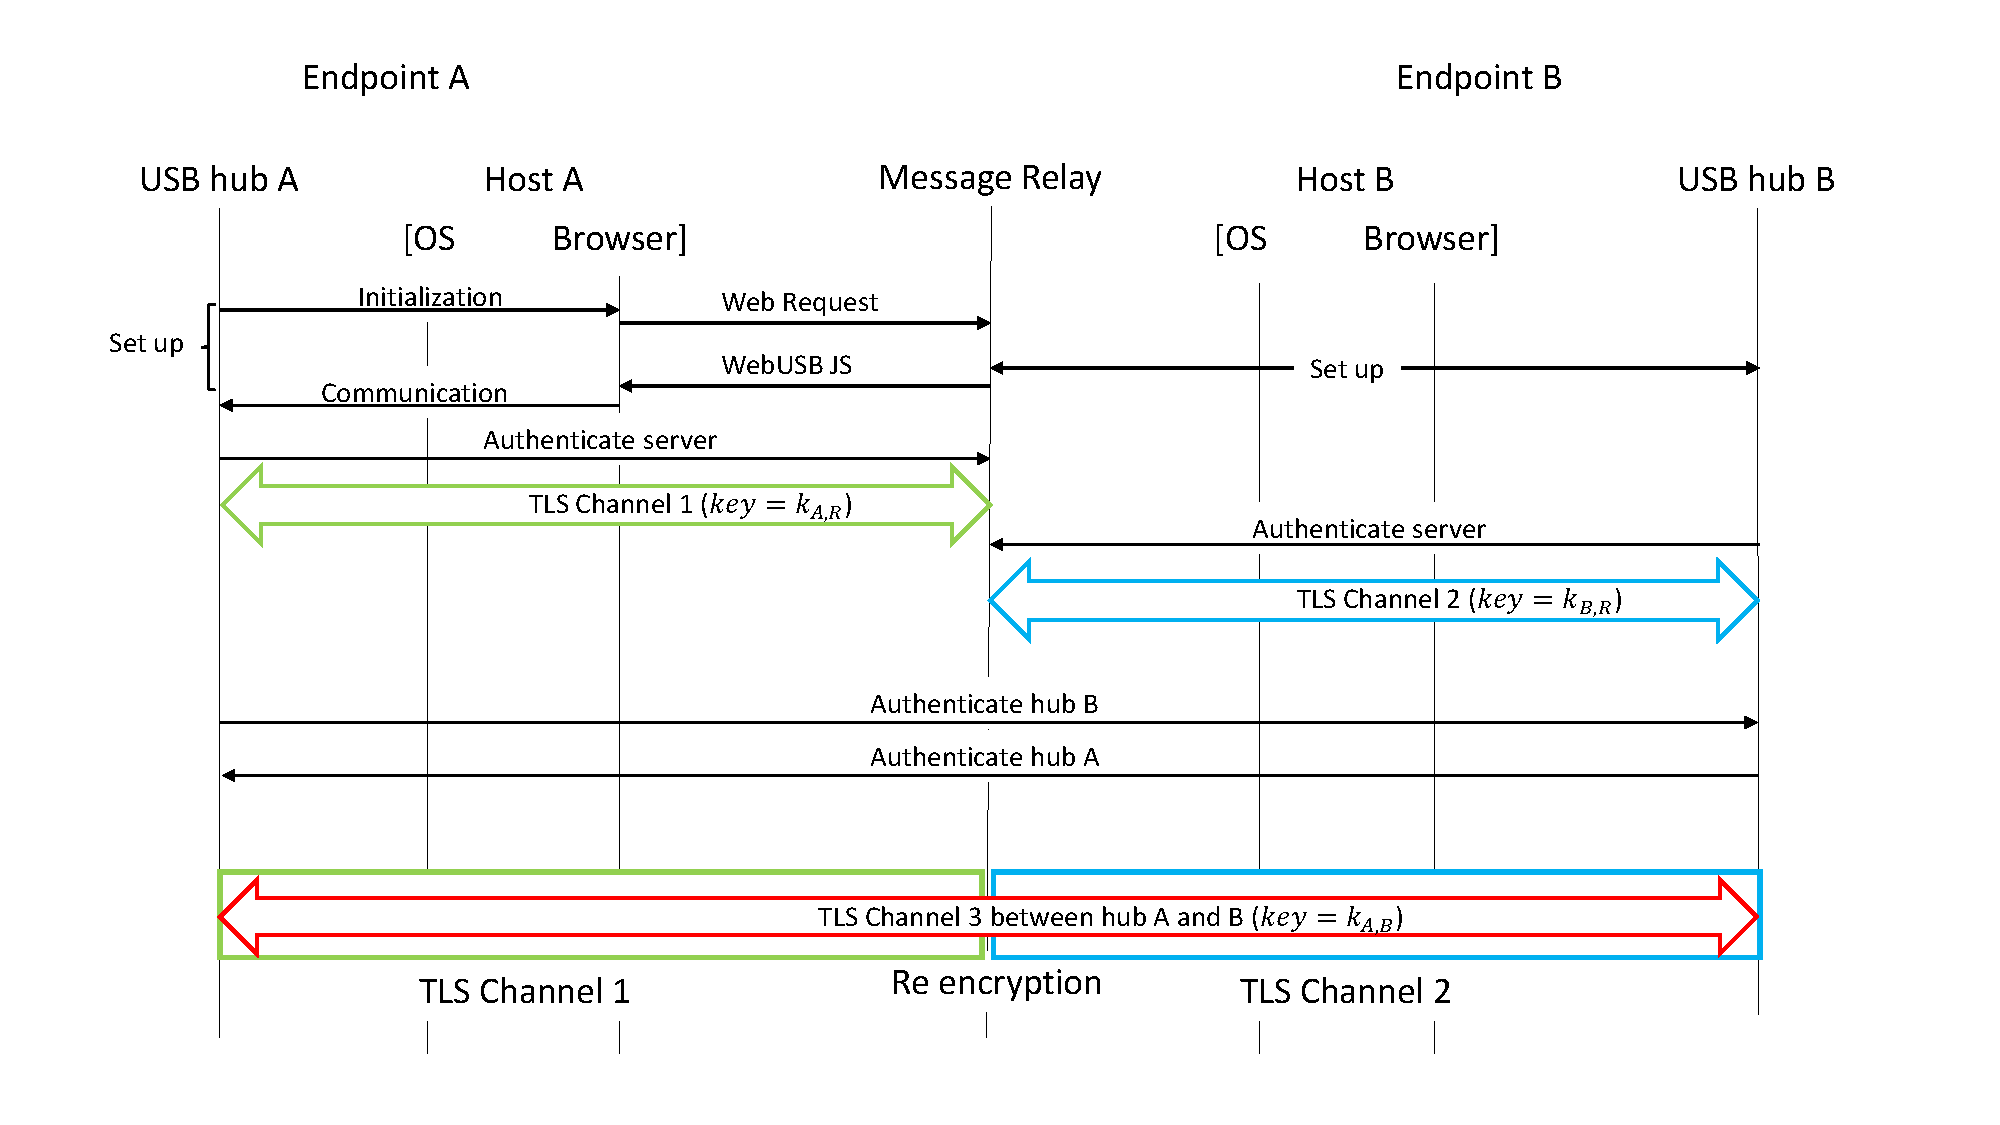
\includegraphics[trim={3cm 1cm 2cm 1cm},width=\linewidth]{interaction.pdf}
 \caption{Interaction diagram between two secure \usb devices A and B (the high-level system diagram is depicted in Figure~\ref{fig:systemDesignDedicated}). This figure4 shows the device to device communication (Section~\ref{sec:secureMessage:deviceToDevice}). An endpoint consists of a secure \usb device, peripheral devices such as a keyboard and a untrusted host system. The browser and the operating system of the host are fully compromised by a global attacker who also has the precise view of the entire network. Here $A$ wants to transfer a message to $B$ and thus initiate a secure channel between $A$ and \relay, similarly secure channel is established between $B$ and \relay. Finally using these two secure channels, $A$ and $B$ establishes a secure channel to deliver the messages.}
 \label{fig:interaction}
\end{figure*}



\begin{figure*}[t]
 \centering
 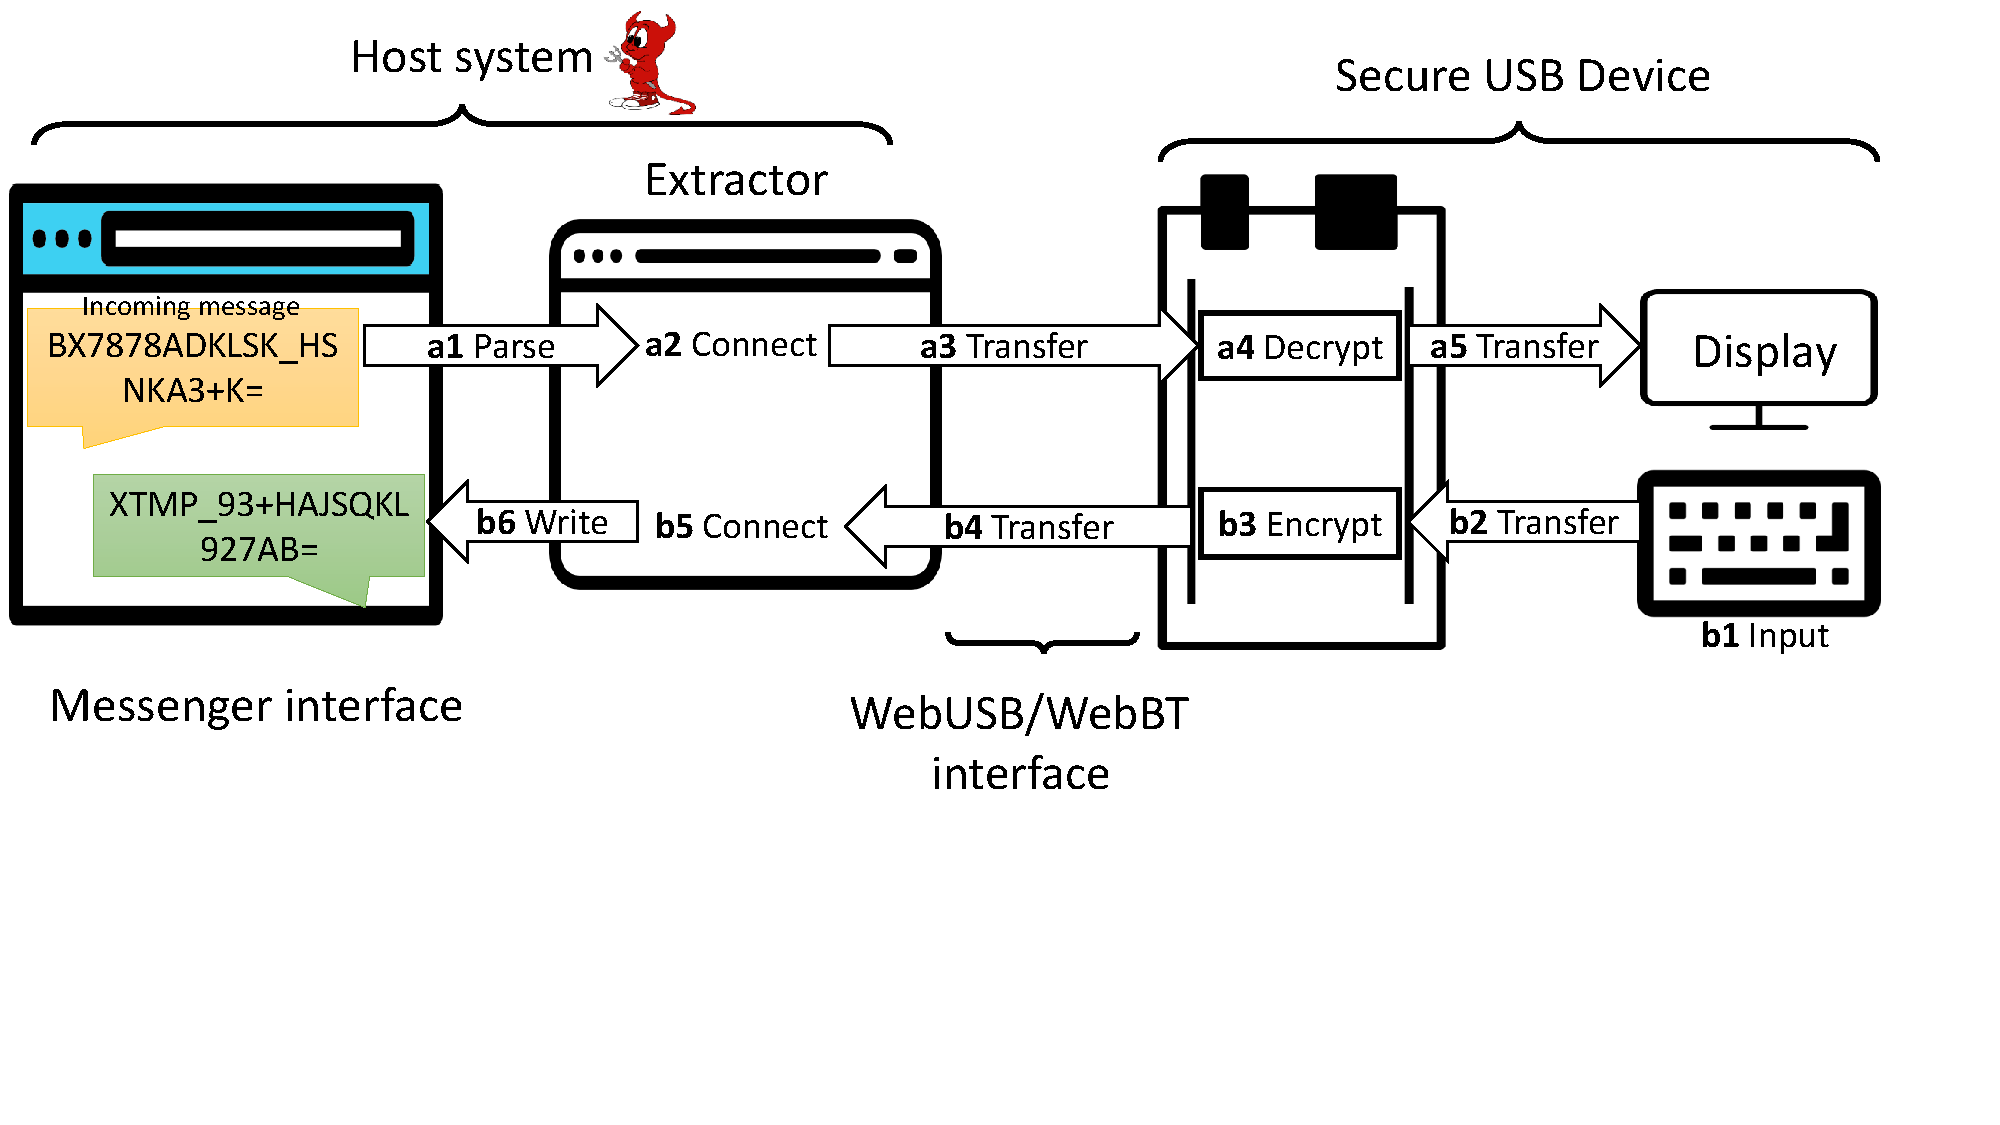
\includegraphics[trim={0 6cm 3cm 0},width=\linewidth]{SystemDesign_Existing.pdf}
 \caption{System design of the secure messaging with existing messenger service. The diagram depicts how messages from the messenger get transferred and decrypted to the secure \usb device display (steps $a1$-$a5$) and the user messages from the device to the messenger (steps $b1$-$b6$). The message interface denotes to the type of application the interface implements such as web interface or browser application or a standalone application. Depending on the message interface the extractor can be designed which can be a browser extension or a standalone application. The extractor uses \webusb/\webbt based serial communication with the secure \usb device. The \usb device has a small display unit and is connected to input peripheral devices such as a keyboard. Note that the message interface and the extractor both are executed on the host system that is fully compromised by the attacker. Any communication between the extractor program and the secure \usb device is carried out by a \usb serial channel. This channel can be wire/wireless and implemented using \webusb/\webbt API.}
 \label{fig:systemDesignExistingMessenger}
\end{figure*}


\subsection{Device to device message relay}
\label{sec:secureMessage:deviceToDevice}

We design and develop an end-to-end secure messaging protocol based on the secure \usb device we developed. The system involves the \usb devices to be present at the sender and the receiver side and a web server that works as a relay (we denote this as \relay). \relay serves \webusb compliant \js snippet to connect with the \usb device and relay the encrypted message from the sender device to the receiver. This setting requires no trust assumption except the certificate authority to issue correct client certificates to the devices. We leverage the existing public key infrastructure (PKI) to issue and manage keys to the client devices. The intermediate relay server (\relay) can also act as the PKI verifier which can notify devices about revokes/renewed certificates and push critical updates to the devices. Figure~\ref{fig:systemDesignDedicated} provides the high-level view of the protocol using a semi-trusted dedicated message relay. The messaging protocol proceeds as the following


\begin{enumerate}

\item The user initializes the secure \usb device that connects with the browser by executing keyboard commands (step $1$ of Figure~\ref{fig:systemDesignDedicated}). This enables the browser to dispatch a \texttt{HTTP} request (step $2$ of Figure~\ref{fig:systemDesignDedicated}) to \relay.
  
\item Upon receiving such request \relay serves the webpage (step $3$ of Figure~\ref{fig:systemDesignDedicated}) that contains a \js that uses \webusb API to connect with the \usb device (step 4).

\item Upon receiving the connection request, the \usb device asks \relay the public certificate and issues challenges to solve. \relay may also send additional challenges to check the client certificate. After the challenge-response messages executed successfully, the device and \relay establishes a \ssl/\tls channel (step $5-8$ of Figure~\ref{fig:systemDesignDedicated}). 

\item We assume that there are two users $A$ and $B$ (as in the Figure~\ref{fig:interaction}). The session secret key between $A$ and \relay is $k_{A, relay}$. 

\item The user $A$ can enter a specific address (which represents another user $B$) to chat with. User $B$ also executes similar challenge response with \relay and establishes a session secret $k_{B, relay}$ (additional information in the figure~\ref{fig:interaction}). 

\item Using these two secure channels (from $A$ to \relay and $B$ to relay through their respective untrusted host systems), $A$ and $B$ exchange challenge messages to verify each other's identities. After that, the two devices at both ends establishes another \ssl/\tls channel inside the former one (between the device and \relay). This secure channel establishment is initiated by the device that wants to talk to the recipient device. All the \ssl/\tls messages are passes through the previously established \ssl/\tls channel between $A$, \relay and $B$, \relay. 

\item After successfully establishing the secure channel, $A$ and $B$ can send and receive encrypted messages (steps $9-15$ of Figure~\ref{fig:systemDesignDedicated}). Figure~\ref{fig:interaction} provides the interaction diagram between two endpoint devices $A$ and $B$ and how \relay handles the secure channel between them.

\end{enumerate}

Figure~\ref{fig:interaction} provides the detailed interaction of device to device messaging (secure \usb device $A$ to $B$) from one untrusted host system to another. 

\subsubsection{Message structure}

Here we specify the message structure of the secure device to device messaging. We assume two users $A$ and $B$ as the sender and the receiver respectively with long-term public-private key pairs $\{PK_A, SK_A\}$ and $\{PK_B, SK_B\}$ respectively. Assume $k_{A,B}$ be the session key established between $A$ and $B$. $A$ construct the following message blob $MB$ for a message $M$ where
%$$MB \leftarrow B | Enc_{k_{A, B}} | Sign{SK_A} $$

\[
  MB \leftarrow 
    \underbrace{Enc_{k_{A, B}} (M)}_{\text{Encrypted Message = C}} | 
    \underbrace{TS}_\text{Timestamp} |
    \underbrace{Sign_{SK_A}(A| B| C | TS)}_\text{Signature}
\]

This is message is transferred through the \tls channel $3$ which is established between $A$ and $B$ (see Figure~\ref{fig:interaction}).

This message blob $MB$ is delivered in encrypted format $C_{A, relay}$ from the user $A$ to the \relay via the \tls channel $1$ (refer to Figure~\ref{fig:interaction}) in the following format:

\[
    C_{A, relay} \leftarrow
    B | 
    \underbrace{Enc_{k_{A, relay}} (MB)}_\text{Encrypted MB = C} |
    \underbrace{Sign_{SK_{A}}(C)}_\text{Signature}
\]
\relay keeps a hash table in its memory which consists of the receiver address and the corresponding encrypted message as a key-value pair. Upon receiving the message $C_{A, relay}$, \relay decrypts it and verify the authenticity by checking the digital signature. Then \relay makes a new entry to the table as $(B, MB)$. In case there exist multiple messages between $A$ and $B$, \relay sorts the messages based on the timestamp of arrival. This was we ensure that the message order is preserved.

When user $B$ comes online, \relay delivered $MB$ by establishing \tls channel $2$ (refer to Figure~\ref{fig:interaction}) as $Enc_{k_{B, relay}} (MB)$ where $k_{B, relay}$ is the session secret key of the \tls connection between $B$ and \relay. Upon receiving this message, $B$ decrypts it and recover $MB$. Then $B$ checks the signature of the message embedded in $MB$ and verifies that the message is actually coming from sender $A$. After that $B$ decrypts the message contains. All of these operations are executed by the \usb device at the end-point $B$ in fully automated manner. 

\subsubsection{Role of the relay server (\relay)}

We introduce the relay server \relay to establish an end-to-end secure messaging channel that provides input integrity and confidentiality. \relay plays several roles in establishing the secure messaging channel between two endpoints. We call endpoint to the users with the untrusted host connected with the secure \usb device.

\begin{itemize}
  \item \relay serves \webusb \js to the users which allow the browser to communicate with the \usb device. This makes the setup process extremely simple and requires the installation of no additional components.
  \item \relay also acts as the certificate authority (CA) which is used to authenticate and establish a secure channel (\ssl/\tls) between the users. \relay can revoke and renew the certificates from where the \usb device update itself. This was \relay serves as a directory server for the messaging channel to establish. The user can find the certificate of other users and authenticate them easily. 
  \item More importantly, \relay works as a message relay to transfer the encrypted messages between the users. \relay keeps a hash table to keep the encrypted message corresponding to the receiver address and deliver them. As \relay handles all the network communications of the users, it exactly knows who talks to whom. But due to the message encryption, \relay does not know the message content. This can be solved by using an ORAM on \relay but that would increase the computational requirement both at \relay and the users.
\end{itemize} 

\subsubsection{Trust assumption}

We assume that the network and the host system (operating system and hardware) is compromised by the attacker. We only trust the \toolname secure \usb device and the relay server (\relay) is semi-trusted. We rely on \relay's certificate to initiate the connection with another device for communication. But as the individual messages are encrypted, \relay does not learn the content of the messages.


\subsection{Secure channel over existing messenger}
\label{sec:secureMessage:existingMessgenger}

An existing messenger service such \emph{WhasApp}, \emph{Signal}, \emph{Telegram} etc. provides an insecure transport channel for the \usb device to communicate securely. Even though most of the messaging services we used to leverage as a transport channel provides strong security guarantees but input confidentially and integrity is not ensured. As our attacker model assumes that the attacker can completely compromise the host system and the network completely, they can easily capture all inputs and read-out all the information displayed on the host system side. Moreover, state nation level attacker may successfully extract communication transcript from the messaging services.

Figure~\ref{fig:systemDesignExistingMessenger} provides overall system design of the end-to-end input secure messenger over existing messaging services. We now generalized our solution by introduction three components

\mypara \textbf{Messenger interface} is the interface where the users interact with the existing messenger. There could be several types of interface such as web-based (WhatsApp, WeChat), browser application based (Signal) or completely standalone (Line, Skype).

\mypara \textbf{Extractor} is a component installed on the host system that can interact with the messenger interface and the secure \usb device. Design of the extractor is dependent on the type of the message interface. For example, if the messenger is a web-based interface then the extractor could be a browser application.
  
\mypara \textbf{Secure \usb device} is the similar \usb device that contains a small display unit and connects with any \usb based peripherals. Ideally, this device should be a small embedded device with the small code base and has enough computation power to establish a \ssl/\tls channel with a remote server.  


%In this settings we leverage existing messenger service as an insecure channel to deliver the messages. 
We implemented the prototype on WhatsApp web interface (\url{web.whatsapp.com}). Here the \emph{message interface} is a web interface written in \texttt{HTML} and \js. The prototype implementation also involves a Google Chrome extension and a chrome packaged application as the \emph{extractor} to communicate with the \usb device. We require both chrome extension and packaged application due to Chrome's separation of privileges policy. An external application has full access to the web page (via a \js code called content script) but it can not communicate to any external application or device (e.g. serial communication). On the other hand, a chrome packaged application can access \usb device via the Chrome \serial API but it has no access to the webpage. Additionally, the chrome extension and the packaged application can communicate via the messaging API. This way we can establish a bi-directional communication channel between the webpage and the \usb device. Alternatively one can eliminate the need of the packaged application by injecting \webusb/\webbt scripts to the main site via the chrome extension. The \webusb/\webbt enabled script can communicate with the secure \usb device directly.

Figure~\ref{fig:systemDesignExistingMessenger} provides the overall flow of the messaging system based on the existing messenger. The proposed solution works as the following:

\begin{enumerate}
  \item When the user selects a contact from the WhatsApp's web interface, the \usb device communicate with the webpage via the extension and the packaged application and compose messages for \ssl/\tls key exchange and put them as a message (\texttt{Base64} encoded string format).
  \item Wen the user receives such encoded message, he clicks on the message bubble. The \usb device capture the chatbox and do the Diffie-Hellman key exchange (step $a1$ of Figure~\ref{fig:systemDesignExistingMessenger}). The key exchange happens in the following way: the clients generate session keys and sign the public key with his long-term private key. The \usb device then converts this information in \texttt{Base64} encoded string and put them in the text box. Upon receiving such message, the browser extension program at the other side capture the chat box and extract the keys and signature from there. Upon verification, the \usb device at the other side does the same. This way the sender and the receiver establishes a secure channel over WhatsApp.
  \item When the user wants to send a message, the user types the message on the keyboard connected to the \usb device which encrypts the message by the session shared secret key established by the aforementioned key exchange. The device then put the encrypted message on the input chat textbox a \texttt{Base64} encode string (steps $b2 - b6$ of Figure~\ref{fig:systemDesignExistingMessenger}).
  \item The receiving mechanism is similar, after receiving an encrypted message, the user simply clicks on the chat bubble. This action allows the \usb device to capture the encrypted message. The device then decrypts the message and shows on the attached display panel (steps $a1 - a5$ of Figure~\ref{fig:systemDesignExistingMessenger}).
\end{enumerate}

\ad{Extend these points later on}

\subsubsection{Role of the existing messenger}
Here we mention the roles of the existing messaging service (we call it as \messenger).

\myparapara{Primary user authentication} Almost all the existing messaging services posses basic authentication scheme either by using a mobile phone number, email address or a combination of such.  
\myparapara{Directory service} As the messaging service already acts as a layer of primary authentication, one can assume it as a directory service provider where the sender can easily find the recipient and execute the key exchange over the messenger to achieve more security.

\myparapara{Reliability} The existing messaging services provide more reliability that ensures that the secure messaging service gets maximum uptime. 


\subsubsection{In-orderness of the messages}

The underlying messaging services ensure the order if delivery of the messages.

\subsubsection{trust assumption}

As our proposed device to device messaging described in Section~\ref{sec:secureMessage:deviceToDevice}, the host system, and the network are fully compromised by the attacker. The existing message service is semi-trusted to provide the correct directory service. Similar to the previous approach, the message service does not know any information about the message content as the individual messages are encrypted.

\subsection{Security properties}
\label{sec:secureMessage:securityProperty}

Now we formally define and analyze the security properties of messaging using the secure \usb device.

\subsubsection{Message confidentiality}

In both of the cases described above (Section~\ref{sec:secureMessage:deviceToDevice} and \ref{sec:secureMessage:existingMessgenger}) message confidentiality is fully preserved from the perspective of the compromised host, network and the existing messaging service. For the device to device message relay (Section~\ref{sec:secureMessage:deviceToDevice}), we can assume that the relay server (\relay) can be honest but curious. This assumption is necessary as at the initialization stage, the \usb device relies on the public certificate of \relay to establish the secure channel using the \webusb enabled \js (served by \relay). This requires trust in the \relay but we can assume that it can be a passive attacker. In both of the proposed methods, the \usb devices at the user sides execute key exchange and establish another secure channel. This makes sure that the \relay has no information about the messages exchanged between the users.

\subsubsection{Message authenticity and integrity}

Message authenticity and integrity is preserved due to the secure channel in both of the protocols. In both cases, the \usb device executes a Diffie-Hellman key exchange by authenticating the public certificate of the device. Additionally, each message is signed by the sender and only accepted after successful verification of the signature, this makes sure that a forged/corrupted message can be detected upon verification. If we assume that the certificate authority is not compromised, message authenticity is trivial.

\subsubsection{Message privacy}
In none of the cases, message privacy is preserved. In both of the cases, the relay and the existing messenger service knows precisely which user is communicating with whom (\ad{for the device to device channel we can solve this by introducing some anonymous credential which can be pseudorandom for every connection}).